\documentclass{beamer}

\usepackage{framed}

\usepackage{graphicx}

\begin{document}
\section{Type I and II Error}
%============================================================%
\begin{frame}
\frametitle{Type I and II Error}
\large
\begin{itemize}
\item In a hypothesis test, a type I error occurs when the null hypothesis
is rejected when it is in fact true; that is, H0 is wrongly rejected.
For example, in a clinical trial of a new drug, the null hypothesis
might be that the new drug is no better, on average, than the
current drug; i.e.
\begin{description}
	\item[H0: ] there is no difference between the two drugs on average.
\end{description}

\item A type I error would occur if we concluded that the two drugs
produced different effects when in fact there was no difference
between them.
\end{itemize}
\end{frame}
%============================================================%
\begin{frame}
	\frametitle{Type I and II Error}
	\large
\begin{itemize}
\item The hypothesis test procedure is therefore adjusted so that there is
a guaranteed 'low' probability of rejecting the null hypothesis
wrongly; this probability is never 0.
\item This probability of a type I error can be precisely computed as
\[\Pr(\mbox{type I error}) = \mbox{significance level} = \alpha\]
\item The exact probability of a type II error is generally unknown.
If we do not reject the null hypothesis, it may still be false (a type
II error) as the sample may not be big enough to identify the
falseness of the null hypothesis (especially if the truth is very close
to hypothesis).
\end{itemize}
\end{frame}
%============================================================%
\begin{frame}
\frametitle{Type I and II Error}
\large
\begin{itemize}
	\item For any given set of data, type I and type II errors are inversely
	related; the smaller the risk of one, the higher the risk of the other.
	\item A type I error can also be referred to as an error of the first kind.
\end{itemize}
	Type II Error
\begin{itemize}
	\item In a hypothesis test, a type II error occurs when the null hypothesis
	H0, is not rejected when it is in fact false. 
	\item For example, in a clinical
	trial of a new drug, the null hypothesis might be that the new drug
	is no better, on average, than the current drug; i.e.
	H0: there is no difference between the two drugs on average.
\end{itemize}

\end{frame}
%============================================================%
\begin{frame}
	\frametitle{Review of Inference Procedures}
	\large
	\begin{itemize}
\item A type II error would occur if it was concluded that the two drugs
produced the same effect, i.e. there is no difference between the
two drugs on average, when in fact they produced different ones.
A type II error is frequently due to sample sizes being too small.
\item The probability of a type II error is generally unknown, but is
symbolised by β and written
\[P(\mbox{type II error}) = \beta\]
\item A type II error can also be referred to as an error of the second
kind.
\end{itemize}
\end{frame}
%============================================================%
\begin{frame}
\frametitle{Review of Inference Procedures}
\large

\textbf{Summary:}\\
The following table gives a summary of possible results of any
hypothesis test:
\begin{figure}
\centering
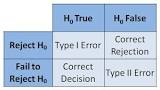
\includegraphics[width=0.6\linewidth]{ErrorTypeTable}

\end{figure}


\end{frame}
%============================================================%
\begin{frame}
\frametitle{Type I and II Error}
\large
\begin{itemize}
\item A type I error is often considered to be more serious, and therefore
more important to avoid, than a type II error. 
\end{itemize}
\textbf{Power}
\begin{itemize}
	\item The power of a statistical hypothesis test measures the test's ability
to reject the null hypothesis when it is actually false - that is, to
make a correct decision.
\end{itemize}
\end{frame}
%============================================================%
\begin{frame}
	\frametitle{Review of Inference Procedures}
	\large
\begin{itemize}
	\item 

In other words, the power of a hypothesis test is the probability of
not committing a type II error. 
\item It is calculated by subtracting the
probability of a type II error from 1, usually expressed as:
\[Power = 1 - P(\mbox{type II error}) = 1- \beta\]
\item The maximum power a test can have is 1, the minimum is 0. Ideally
we want a test to have high power, close to 1.
\end{itemize}
\end{frame}
\section{One Tailed Testing}
%============================================================%
\begin{frame}
\frametitle{Review of Inference Procedures}
\large
\noindent \textbf{One Tailed Testing}
\begin{itemize}
	\item A one-sided test is a statistical hypothesis test in which the values
	for which we can reject the null hypothesis, H0 are located entirely
	in one tail of the probability distribution.
	\item In other words, the critical region for a one-sided test is the set of
	values less than the critical value of the test, or the set of values
	greater than the critical value of the test.
\end{itemize}


\end{frame}
%============================================================%
\begin{frame}
\frametitle{Review of Inference Procedures}
\large
\begin{itemize}
	\item We generally use it to formally test whether a parameter value is
	greater or less than some specified value, or for the case of two
	samples, if the parameter values from sample is greater or less
	than the corresponding parameter value from the other sample.
	\item A one-sided test is also referred to as a one-tailed test of
	significance.
\end{itemize}


\end{frame}
%==========================================================================================%
\begin{frame}
\frametitle{Titration experiment}
	
Four Students, A,B,C and D performing the same experiment five times, hence each yield 5 results.%(Table 1.1 random and systematic errors).

	\begin{tabular}{|c|ccccc|l|}
		\hline
		% after \\: \hline or \cline{col1-col2} \cline{col3-col4} ...
		 & Results  & (ml) &  &  &  &Comment \\ \hline
		A & 10.08 & 10.11 &10.09 &10.10&10.12 & Precise, biased\\ \hline
		B & 9.88 &10.14& 10.02 &9.80& 10.21& Imprecise unbiased\\ \hline
		C & 10.19 &9.79& 9.69 &10.05& 9.78 & Imprecise, biased\\ \hline
		D & 10.04 &9.98 &10.02 &9.97 &10.04 & Precise, unbiased \\
		\hline
	\end{tabular}\\
\end{frame}
%==========================================================================================%
\begin{frame}
	\frametitle{Titration experiment}
	
\begin{itemize}
\item	Two criteria were used to compare these results, the average value (technically know
	as a measure of location and the degree of spread (or dispersion). 
\item The average value
	used was the arithmetic mean (usually abbreviated to \emph{the mean}), which is the sum
	of all the measurements divided by the number of measurements.	
\end{itemize}	

	
\end{frame}
%==========================================================================================%
\begin{frame}
	\frametitle{Titration experiment}	
	The mean,$\bar{X}$, of $n$ measurements is given by \[ \bar{X}  = {\sum{x} \over n} \]
	
	In Chapter 1 the spread was measured by the difference between the highest and
	lowest values (i.e. the range). A more useful measure, which utilizes all the values, is the sample
	standard deviation, $s$, which is defined as follows:
	
	The standard deviation, $s$, of $n$ measurements is given by
	\[s=  \sqrt{ {\sum(x-\bar{X})^2 \over n-1} }  (2.2) \]
\end{frame}
%============================================================%
\begin{frame}[fragile]
\frametitle{Review of Inference Procedures}
\large
The choice between a one-sided and a two-sided test is determined
by the purpose of the investigation or prior reasons for using a onesided
test.
%Recall the titration experiments from the previous week:
\begin{verbatim}
A 10.08 10.11 10.09 10.10 10.12
B  9.88 10.14 10.02  9.80 10.21
C 10.19  9.79  9.69 10.05  9.78
D 10.04  9.98 10.02  9.97 10.04
\end{verbatim}
We shall perform a series of one sample and two sample tests.
Recall the true value of the titration experiment in each case is
supposed to be 10.
First we will consider the case of A’s measurements ( as we did in
the previous lecture).
\end{frame}
%============================================================%
\begin{frame}[fragile]
	\frametitle{Review of Inference Procedures}
The mean and standard deviation of A’s measurements are as
follows:
\begin{framed}
\begin{verbatim}
> mean(X.A)
[1] 10.1
> sd(X.A)
[1] 0.01581139
\end{verbatim}
\end{framed}
We will perform two one-tailed tests. To recap, we performed a two
tailed test in the previous lecture (i.e. the true mean is equal to
zero). To contrast with the one-tailed tests, here is it again, with
the alternative specified.

\end{frame}
%============================================================%
\begin{frame}[fragile]
\frametitle{Review of Inference Procedures}
\large
\begin{framed}
\begin{verbatim}
> t.test(X.A, mu=10, alternative = "two.sided")
One Sample t-test
data: X.A
t = 14.1421, df = 4, p-value = 0.0001451
alternative hypothesis: 
		true mean is not equal to 10

95 percent confidence interval:
10.08037 10.11963
sample estimates:
mean of x
 10.1
\end{verbatim}
\end{framed}
\end{frame}
%============================================================%
\begin{frame}[fragile]
	\frametitle{Review of Inference Procedures}
	\large
We will perform a “greater than” test. The null and alternative are
specified as follows:
\begin{description}
	\item[H0:] $μA \leq 10$ True value of population mean is no more than 10
	\item[H1:] $μA > 10$ True value of population mean is greater than 10.
\end{description}


\end{frame}
%============================================================%
\begin{frame}[fragile]
\frametitle{Review of Inference Procedures}
\large
\begin{verbatim}
> t.test(X.A, mu=10, alternative = "greater")
 One Sample t-test
data: X.A
t = 14.1421, df = 4, p-value = 7.256e-05
alternative hypothesis: true mean is greater than 10
95 percent confidence interval:
10.08493 Inf
sample estimates:
mean of x
 10.1
\end{verbatim}
\end{frame}
%============================================================%
\begin{frame}
\frametitle{Review of Inference Procedures}
\large
In this case, we would reject the null hypothesis, based on the
extremely low p-value. There is very convincing evidence to say
that the true mean of A’s measurements is greater than 10.
(Furthermore there is a systematic upward bias in A’s
measurements)
\end{frame}
%============================================================%
\begin{frame}
	\frametitle{Review of Inference Procedures}
	\large
Now we will perform a “less than” test. The null and alternative are
specified as follows:
\begin{description}
	\item[H0:] $\mu_A$ $geq$ 10 True value of population mean is at least 10
	\item[H1:] $\mu_A$ $<$ 10 True value of population mean is less than 10.
\end{description}

\end{frame}
%============================================================%
\begin{frame}[fragile]
	\frametitle{Review of Inference Procedures}
	\large
\begin{verbatim}
> t.test(X.A, mu=10, alternative = "less")
 One Sample t-test
data: X.A
t = 14.1421, df = 4, p-value = 0.9999

alternative hypothesis: true mean is less than 10
95 percent confidence interval:
 -Inf 10.11507
sample estimates:
mean of x
 10.1
 \end{verbatim}
 
In this case, we would fail to reject the null hypothesis, based on
the extremely high p-value.
\end{frame}
%============================================================%
\begin{frame}[fragile]
	\frametitle{Review of Inference Procedures}
	\large

\noindent \textbf{Example: Two Sample Testing}
In the previous class, we discussed the test of equality of population
mean for two independent samples.
Let us use the measurements from Students A and B. The mean
and standard deviation of B’s measurements are as follows:
\begin{framed}
\begin{verbatim}
> mean(X.B)
[1] 10.01
> sd(X.B)
[1] 0.1717556
\end{verbatim}
\end{framed}
The hypotheses can be stated as follows:
\begin{description}
	\item[H0:] $\mu_A =\mu_B $ Population means are equal for students A and B
	\item[H1:] $\mu_A \neq \mu_B $ Population means are not equal for A and B
\end{description}
 
\end{frame}
%============================================================%
\begin{frame}[fragile]
	\frametitle{Review of Inference Procedures}
	\large
	To implement such as test in R, we simply specify both data sets.
\begin{framed}
\begin{verbatim}
> t.test(X.A, X.B)
 Welch Two Sample t-test
data: X.A and X.B
t = 1.1668, df = 4.068, p-value = 0.3071
alternative hypothesis: true difference in means is not equal to 0
95 percent confidence interval:
-0.1227643 0.3027643
sample estimates:
mean of x mean of y
 10.10 10.01
 \end{verbatim}
 \end{framed}
Based on the p-value, we fail to reject the null hypothesis.
Note the name given to the output of the procedure “ Welch Two
Sample t-test”.

\end{frame}
%============================================================%
\begin{frame}[fragile]
\frametitle{Review of Inference Procedures}
\large
\begin{itemize}
	\item There are in fact two different two-sample t-tests that can be
	implemented in R.
	\item The test that we have just completed, i.e. the Welch test, does not
	make the assumption that both data sets have equal variance.
	\item Conversely, the “Student Two Sample t-test” does make that
	assumption when performing the test.
\end{itemize}

\end{frame}
%============================================================%
\begin{frame}[fragile]
	\frametitle{Review of Inference Procedures}
	\large
	To perform a Student Two Sample t-test using R, we must
additionally specify that the variances are assumed to be equal
\begin{verbatim}
> t.test(X.A, X.B, var.equal =TRUE)
Two Sample t-test
data: X.A and X.B
t = 1.1668, df = 8, p-value = 0.2769
alternative hypothesis: true difference in means is not equal to 0
95 percent confidence interval:
-0.0878765 0.2678765
sample estimates:
mean of x mean of y
     10.10     10.01
\end{verbatim}

In this instance, we would come to the same conclusion whether or
not we specify the assumption of equal variances.
Notice, however, the p-value and confidence intervals are quite
different.
\end{frame}
%============================================================%
\begin{frame}
	\frametitle{Review of Inference Procedures}
	\large
	In some instances, it is possible that a null hypothesis would be
rejected by one test, but not by the other.

\end{frame}
\section{Formal Test for Equality of Variances}
%============================================================%
\begin{frame}
	\frametitle{Review of Inference Procedures}
	\large
\noindent{Formal Test for Equality of Variances}
R provides us with a formal test for equality of variances for two
samples.

The hypotheses can be stated as follows:
\begin{description}
	\item[H0:] $\sigma^2_A = \sigma^2_B$ Population variances are equal for A and B
	\item[H1:] $\sigma^2_A \neq \sigma^2_B$ Population variances are not equal for A and B
\end{description}


\end{frame}
%============================================================%
\begin{frame}
	\frametitle{Review of Inference Procedures}
	\Large
	Specifically, R considers the ratio of the variances. If two
populations have equal variance, then this variance ratio is one.
The hypotheses can be re-stated as follows:

\begin{description}
	\item[H0:] $\sigma^2_A / \sigma^2_B = 1 $ Population variances ratio is 1
	\item[H1:] $\sigma^2_A / \sigma^2_B \neq 1$ Population variances ratio is not 1
\end{description}
\end{frame}
%============================================================%
\begin{frame}[fragile]
	\frametitle{Review of Inference Procedures}
	\Large
To recap – the variances of A’s and B’s measurements are as
follows. Also computed is the ratio of these variances.
\begin{framed}
\begin{verbatim}
> var(X.A)
[1] 0.00025
> var(X.B)
[1] 0.0295
> var(X.A)/var(X.B)
[1] 0.008474576
> var(X.B)/var(X.A)
[1] 118
\end{verbatim}

\end{framed}
\end{frame}
%============================================================%
\begin{frame}[fragile]
\frametitle{Review of Inference Procedures}
\Large

The test is carried out using the var.test() command.
\begin{framed}
	\begin{verbatim}> var.test(X.A, X.B)
 F test to compare two variances
data: X.A and X.B
F = 0.0085, num df = 4, denom df = 4, p-value = 0.0004213
alternative hypothesis: true ratio of variances is not equal to 1
95 percent confidence interval:
0.000882352 0.081394321
sample estimates:
ratio of variances
 0.008474576
\end{verbatim}

\end{framed}
\end{frame}
%============================================================%
\begin{frame}
\frametitle{Review of Inference Procedures}
\large
\noindent \textbf{F-test of equality of variances}
\begin{itemize}
	\item 

Here we reject the null hypotheses. The p-value is extremely small.
\item It doesn’t matter which order the data sets are specified, other than
the fact that it will reciprocate the variance ratio.
\end{itemize}

The test statistic is

\begin{equation} F = \frac{S_X^2}{S_Y^2}\end{equation}

has an F-distribution with $n-1$ and $m-1$ degrees of freedom if the null hypothesis of equality of variances is true.

\end{frame}
%============================================================%
\begin{frame}[fragile]
\frametitle{Review of Inference Procedures}
\large
\begin{framed}
	\begin{verbatim}
> var.test(X.B, X.A)
F test to compare two variances
data: X.B and X.A
F = 118, num df = 4, denom df = 4, p-value = 0.0004213
alternative hypothesis: true ratio of variances is not equal to 1
95 percent confidence interval:
12.28587 1133.33453
sample estimates:
ratio of variances
  118
\end{verbatim}

\end{framed}

Notice the 95\% confidence interval for the variance ratio. We are
95\% confident that this interval contains the true variance ratio
(i.e. we are 95\% confident that the true variance ratio is between
12.28 and 1133.33).

\end{frame}
%============================================================%
\begin{frame}
\frametitle{Review of Inference Procedures}
\Large
\begin{itemize}
	\item We can reject the null hypothesis on the basis that the value of 1 is
	not contained in that interval.
\item 	Referring back to the two-sample t test; the first test i.e. the Welch
	test, did not rely on the equality of variances, so it is the preferred
	procedure in that case.
\item	Summary: before performing a two-sample t test, check to see if
	the assumption of equal variance is valid.
\end{itemize}


\end{frame}
\section{Paired T Test}
%============================================================%
\begin{frame}
\frametitle{Review of Inference Procedures}
\Large
\noindent \textbf{Paired t-test}
A paired t-test is used to compare two population means where
there are two samples in which observations in one sample can be
paired with observations in the other sample.
Examples of where this might occur are:
\begin{itemize}
	\item Before-and-after observations on the same subjects (e.g.
	patient’s diagnostic test results before and after a particular
	course of treatment).
\item A comparison of two different methods of measurement or
	two different treatments where the measurements/treatments
	are applied to the same subjects (e.g. measurements made
	with Ultra Violet Spectroscopy and Near Infrared Reflectance
	spectroscopy).
\end{itemize}


\end{frame}
%============================================================%
\begin{frame}
\frametitle{Review of Inference Procedures}
\Large
The hypotheses can be stated as follows:
\begin{description}
\item[H0:] μdiff =0 Population mean of case-wise differences is zero
\item[H1:] μdiff ≠ 0 Population mean of case-wise differences is not zero
\end{description}
\begin{itemize}
\item The null hypothesis would articulate the argument that a course of
treatment had no effect on the subjects, or for the second case,
that there is no significant measurement bias between two methods
of measurement.
\item We will perform a case study of this in the Lab Classes.
\end{itemize}
\end{frame}
%============================================================%
\end{document}